\documentclass[a4paper,10pt]{article}
\usepackage[a4paper, total={6in, 8in}]{geometry}
\setlength\parindent{0pt}
\usepackage[utf8]{inputenc}
\usepackage{graphicx} 
\usepackage{amsmath}
\usepackage{amsfonts}
\usepackage{amssymb}
\usepackage{listings}
\usepackage{ragged2e}
\usepackage{listings}
\usepackage{color}
\usepackage[table]{xcolor}
\usepackage{soul}
\usepackage[font=small,labelfont=bf]{caption}
\setlength{\parskip}{\baselineskip}%
\setlength{\parindent}{0pt}%

\begin{document}
\begin{titlepage}
	\centering
	
\includegraphics[width=.6\textwidth]{liu-logo.png}\par
	\vfill
	{\scshape\Large TDDD41 Data Mining - Clustering and Association Analysis\par}
	{\huge\bfseries Lab 2 -  Group 4 Report\par}
	\vspace{0.5cm}
    {\large\itshape Lawrence Thanakumar Rajappa (lawra776)\\
     \large\itshape Kyriakos Domanos (kyrdo817)\par}
	\vfill
	{\large \today\par}
\end{titlepage}
\definecolor{dkgreen}{rgb}{0,0.6,0}
\definecolor{gray}{rgb}{0.5,0.5,0.5}
\definecolor{mauve}{rgb}{0.58,0,0.82}

\begin{center}
	\large\textbf{\underline{Association Analysis}} \par
\end{center} \par
\textbf{\underline{Data Preparation}} \par
In this lab assignment, we used iris dataset which contains 50 samples of data which corresponds to three species of
iris. As a starting process, we discretize the data since association analysis in weka cannot be done on continuous
data. This is done by applying discretize filter available in Weka on only first 4 columns and now, the entire data
is converted discrete format. \par
\textbf{\underline{Clustering - SimpleKmeans}} \par
Now, we tried to apply \textbf{\textit{SimpleKmeans}} clustering algorithm with the following specifications;
\begin{enumerate}
  \item[$*$] \textbf{Seed value} $:$ 10
  \item[$*$] \textbf{No. of Clusters} $:$ 3 
\end{enumerate}
and igonred \textbf{\textit{class}} attribute and selected Classes to clusters evaluation to crosstabulate the 
clustering. We tried to visualize the result of clustering and found that with 3 bins, we could see that sepal 
width and length have lower impact when compared with petal width and length which has higher impact in naming
the flower types. This is because, sepal width and length try to overlap more than petal width and length. Please
refer the below images,
\begin{center}
  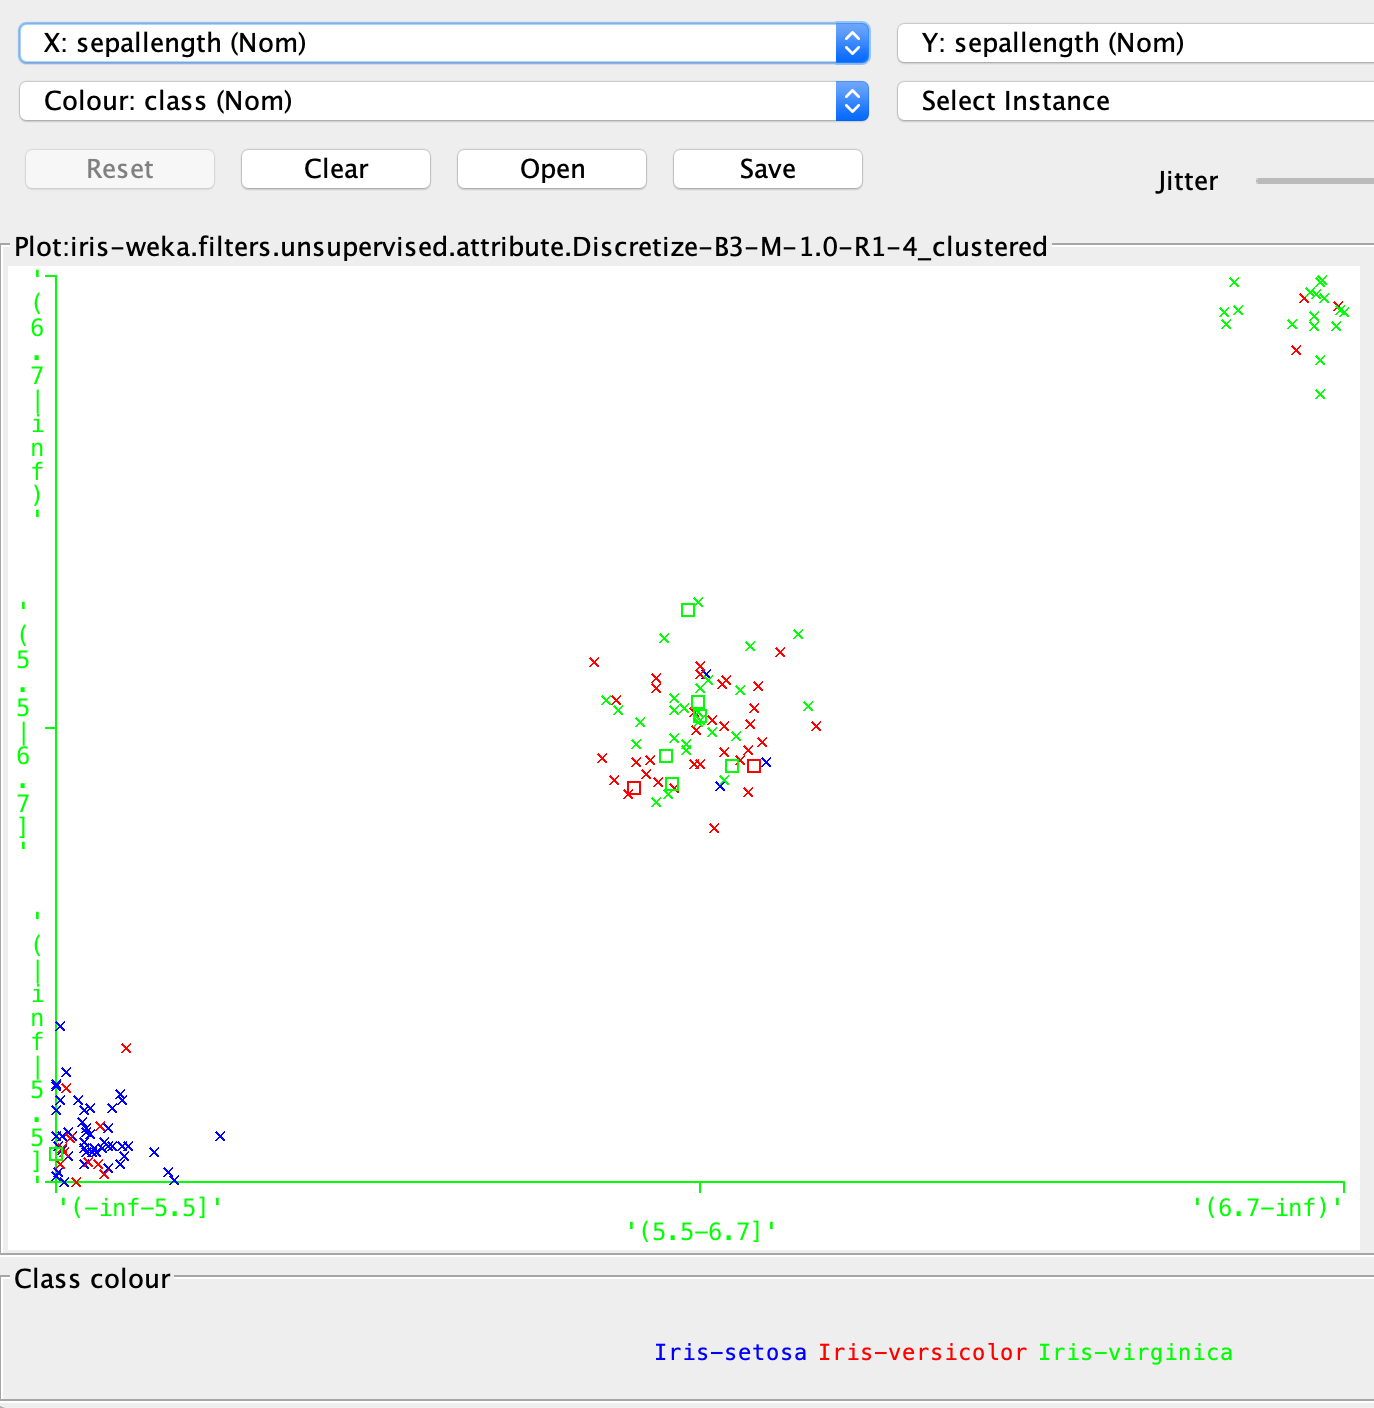
\includegraphics[width=80mm,scale=0.10]{Sepal_dimension_visualization.png}
  \captionof{figure}{Sepal width and length tends to have more overlap in the data}
\end{center}
\par
\begin{center}
  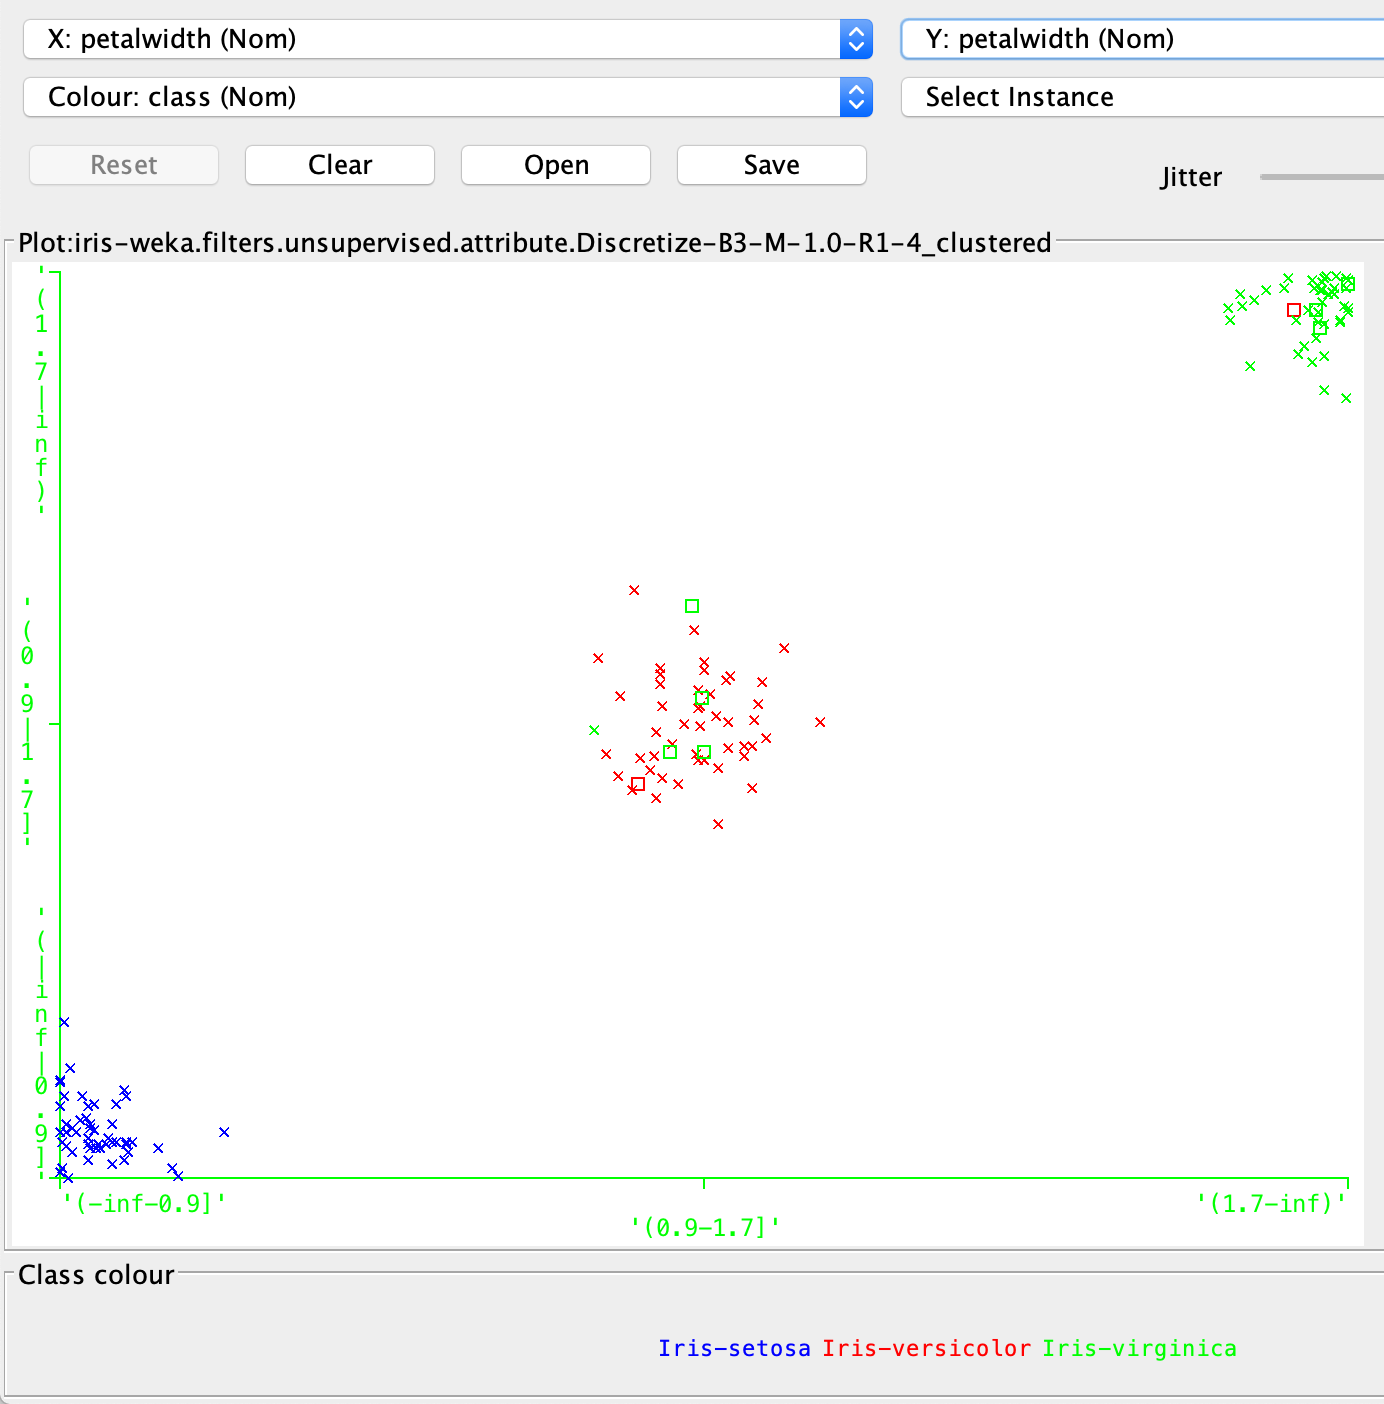
\includegraphics[width=80mm,scale=0.10]{Petal_dimension_visualization.png}
  \captionof{figure}{Petal width and length tends to have less overlap in the data}
\end{center}
and also having less number of bins, we could lose some information as well.
From the clustering result, we could see that clustering has been done well with 3 bins and 3 clusters, \textbf{\textit{iris setosa}}
has been clustered properly and belongs to \textbf{\textit{Cluster 2}}, while there is a swap in case of 
\textbf{\textit{iris versicolor}} and \textbf{\textit{iris virginica}} between \textbf{\textit{Cluster 0}} and
\textbf{\textit{Cluster 1}}.  Please refer to the confusion matrix below, \par
\begin{center}
  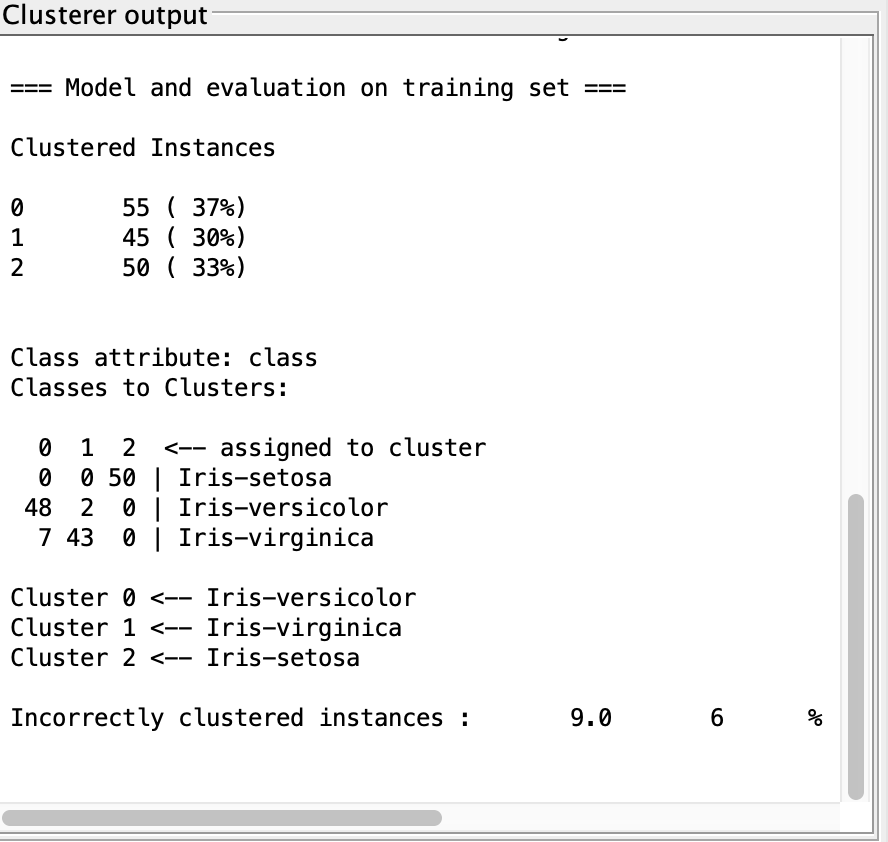
\includegraphics[width=80mm,scale=0.10]{kmeans_clustering.png}
  \captionof{figure}{SimpleKmeans clustering with 3 bins}
\end{center}
Also, if we try to increase the number of bins and discretize, the results are getting worse, please refer the 
image below,
\begin{center}
  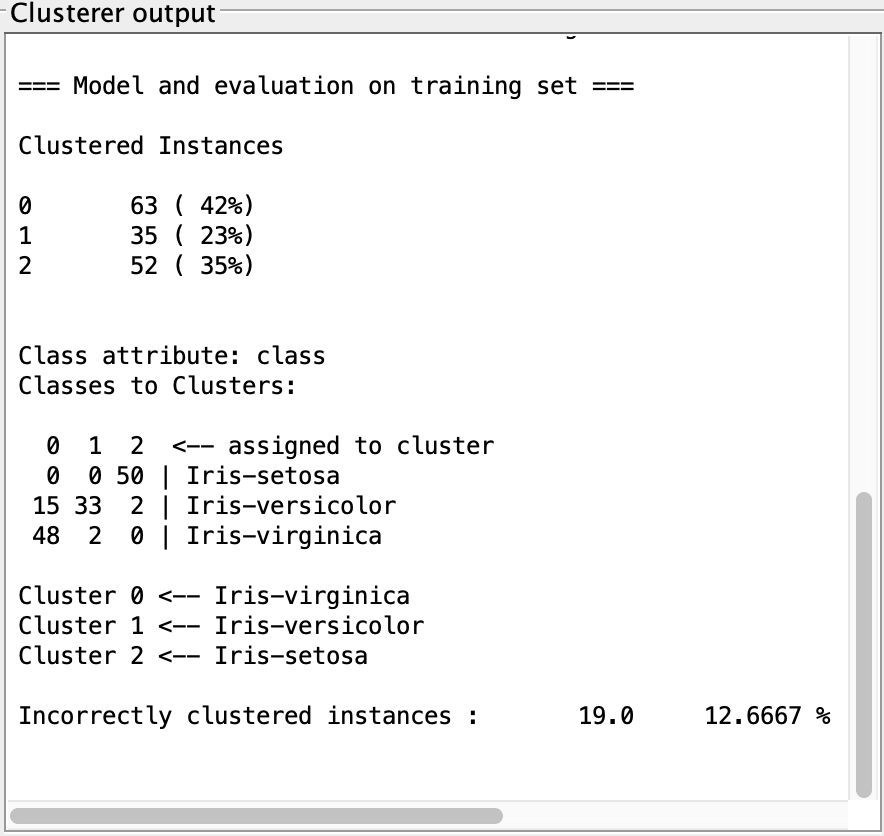
\includegraphics[width=80mm,scale=0.10]{kmeans_clustering_1.png}
  \captionof{figure}{SimpleKmeans clustering with 5 bins}
\end{center}
\par
\textbf{\underline{Association Analysis - Apriori}} \par
Here we have used the following specifications for performing Apriori algorithm on 3 clustered dataset;
\begin{enumerate}
  \item [$*$] \textbf{Minimum Support} = 0.1
  \item [$*$] \textbf{Metric type} = Confidence
  \item [$*$] \textbf{Minimum Confidence} = 0.9
\end{enumerate}
with the above properties, we have performed apriori algorithm on the iris dataset and got the following association rules
which are given below,
\begin{center}
  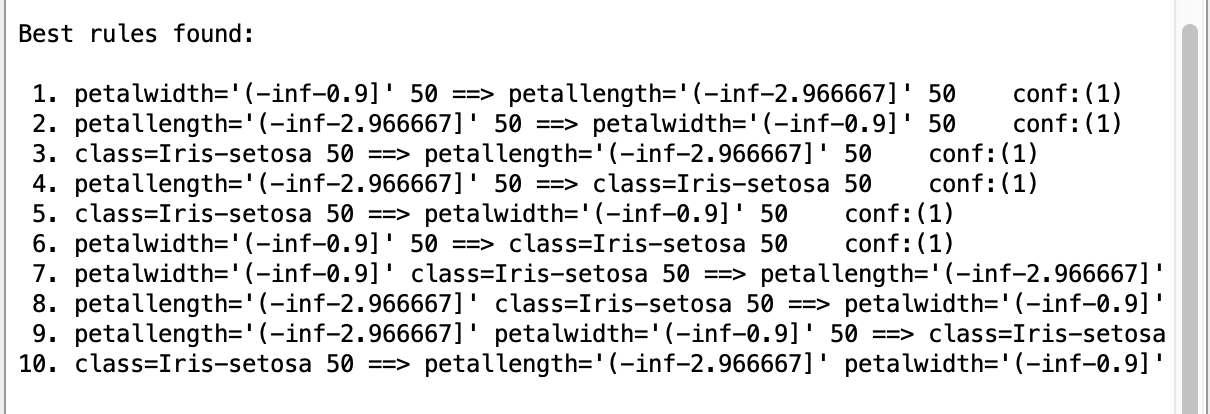
\includegraphics[width=80mm,scale=0.10]{apriori_assoociation.png}
  \captionof{figure}{Apriori - Association Rules with Confidence}
\end{center}
In this frequent itemset are the attribute-value pair and transaction is a single data point. Moreover, with 
default properties we weren't able to get proper association rules, hence we changed our properties a bit;
\begin{enumerate}
  \item [$*$] \textbf{Number of Rules} = 1000
  \item [$*$] \textbf{Metric type} = Confidence
  \item [$*$] \textbf{Minimum Confidence} = 0.9
\end{enumerate}
In the above properties, \textbf{\textit{Number of Rules}} which specifies how many rules are needed and we get
1000 rules from this property and we keep the rule with 90\% confidence.
\begin{enumerate}     
  \item [$*$] sepalwidth='(-inf-2.8]' petallength='(2.966667-4.933333]' ==$>$ Cluster=cluster1, Occurrence = 30, Confidence:(1)
  \item [$*$] petallength='(2.966667-4.933333]' petalwidth='(0.9-1.7]' ==$>$ Cluster=cluster1, Occurrence = 48, Confidence:(1)
  \item [$*$] petallength='(4.933333-inf)' petalwidth='(1.7-inf)' ==$>$ Cluster=cluster2, Occurrence = 40, Confidence:(1)
  \item [$*$] sepallength='(6.7-inf)' petallength='(4.933333-inf)' ==$>$ Cluster=cluster2, Occurrence = 17, Confidence:(1)
  \item [$*$] sepallength='(-inf-5.5]' petallength='(-inf-2.966667]' ==$>$ Cluster = cluster3, Occurrence = 47, confidence:(1)
  \item [$*$] sepalwidth='(2.8-3.6]' petallength='(-inf-2.966667]' ==$>$ Cluster=cluster3, Occurrence = 36, Confidence:(1)
\end{enumerate}
\par
From the above association rules, we could see that we want class to be in consequent rather than in antecedent, because
we need to predict the class of the flower and also when a new data comes into the system, we need to predict its species
instead of having the class at beginning and attributes are placed in consequent because it is not to be predicted. \par
\textbf{\underline{Experiments}} \par
\textbf{\underline{Different Number of Bins}} \par
By increasing number of bins, we could yield more information and thus we can calculate distance between data points 
more precisely in k-means algorithm. On the other hand, having to many clusters which would yield less information and
possibly it could make the algorithm ambiguous. 

We tried to discretize the data with \textbf{\textit{6 bins}} and found that the amount of incorrectly clustered
data points are more when compared with the clustering result with 3 bins, which makes the above line true. We then
applied \textbf{\textit{addCluster}} filter on the 6 bins data and found the following association rules;
\begin{enumerate}
  \item [$*$] petallength='(-inf-1.983333]' ==$>$ cluster=cluster1 occurrence = 50    conf:(1)
  \item [$*$] petalwidth='(-inf-0.5]' ==$>$ cluster=cluster1 occurrence = 49    conf:(1)
  \item [$*$] sepallength='(5.5-6.1]' petallength='(3.95-4.933333]' ==$>$ cluster=cluster2 occurrence = 21    conf:(1)
  \item [$*$] petallength='(3.95-4.933333]' petalwidth='(0.9-1.3]' ==$>$ cluster=cluster2 occurrence = 18    conf:(1)
  \item [$*$] sepallength='(6.1-6.7]' petallength='(4.933333-5.916667]' ==$>$ cluster=cluster3 occurrence = 20    conf:(1)
  \item [$*$] sepalwidth='(2.8-3.2]' petallength='(4.933333-5.916667]' ==$>$ cluster=cluster3 occurrence = 18    conf:(1)
\end{enumerate}
From the association rules above, we infer that cluster1 is characterized by only petal length and petal width, while
cluster2 and cluster3 are characterized by mix of attribute values. This clustering is not good because there is 20.6667\% 
of incorrectly clustered instances. This is because some of the values don't reach the minimum support and don't
give rise to correct rules. From this we can conclude that instead of increasing the bins, we can perform discretize
in an efficient way.
\par
\textbf{\underline{Different Number of Bins}} \par
\end{document}

